\documentclass[aspectratio=169,10pt]{beamer}

\usetheme{Madrid}
\usecolortheme{seahorse}

% Packages
\usepackage[utf8]{inputenc}
\usepackage[T1]{fontenc}
\usepackage{amsmath, amssymb, amsfonts}
\usepackage{mathtools}
\usepackage{listings}
\usepackage{xcolor}
\usepackage{graphicx}
\usepackage{hyperref}
\usepackage{tikz}
\usepackage{array}
\usepackage{booktabs}
\usepackage{multicol}
\usepackage{xparse}

% Graphics path
\graphicspath{{figures/}}

% Listings style
\lstset{
    basicstyle=\ttfamily\scriptsize,
    keywordstyle=\color{blue},
    commentstyle=\color{green!50!black}\itshape,
    stringstyle=\color{red},
    numbers=left,
    numberstyle=\tiny\color{gray},
    frame=single,
    breaklines=true,
    breakatwhitespace=true,
    tabsize=2,
    showstringspaces=false,
    language=Python,
    inputencoding=utf8,
    extendedchars=true
}

% Define exercise environment
\newenvironment{exercise}{\begin{definition}[Exercise]}{\end{definition}}

% Foot line
\setbeamertemplate{footline}[frame number]

% Title page
\title[Banach Contraction Mapping]{Banach Contraction Mapping Theorem}
\subtitle{Fixed Point Theory and Applications}
\author[Pathak]{Hemant Kumar Pathak\\An Introduction to Nonlinear Analysis and Fixed Point Theory}
\date{\today}
\institute{Lecture Notes on Nonlinear Analysis}

\begin{document}

% Title Slide
\begin{frame}
    \titlepage
    \vspace{0.5cm}
    \begin{center}
        \textbf{Chapter 2b: Banach Contraction Mapping}\\
        Complete Metric Spaces and Fixed Point Theorems
    \end{center}
\end{frame}

% Table of Contents
\begin{frame}[allowframebreaks]{Outline}
    \tableofcontents
\end{frame}

% Section 1: Introduction and Motivation
\section{Introduction and Motivation}

\begin{frame}{What is a Fixed Point?}
    \begin{definition}[Fixed Point]
        Let $T: X \to X$ be a mapping of a set $X$ into itself. An element $x^* \in X$ is called a \textbf{fixed point} (or invariant point) of $T$ if
        \[
            T(x^*) = x^*
        \]
    \end{definition}

    \vspace{0.3cm}
    \begin{example}
        \begin{itemize}
            \item $T(x) = x^2$ on $[0,1]$: fixed points are $x^* = 0$ and $x^* = 1$
            \item $T(x) = \cos(x)$ on $\mathbb{R}$: fixed point exists (approx.~$x^* \approx 0.739$)
            \item $T(x) = 2x$ on $\mathbb{R}$: no fixed points (except if we allow infinity)
        \end{itemize}
    \end{example}

    \vspace{0.3cm}
    \begin{center}
        \textcolor{red}{Central Question:} When does a mapping have a fixed point?
    \end{center}
\end{frame}

\begin{frame}{Motivation: Why Study Fixed Points?}
    Fixed point theorems have profound applications in mathematics and beyond:

    \begin{multicols}{2}
        \begin{itemize}
            \item \textbf{Differential Equations:} Existence and uniqueness of solutions
            \item \textbf{Integral Equations:} Solutions via fixed point iteration
            \item \textbf{Numerical Analysis:} Newton-Raphson, iterative methods
            \item \textbf{Economics:} Market equilibrium, game theory
            \item \textbf{Control Theory:} Optimal control problems
            \item \textbf{Fractional Calculus:} Solutions of fractional ODEs
        \end{itemize}
    \end{multicols}

    \vspace{0.3cm}
    \vspace{0.2cm}
\end{frame}

% Section 2: Complete Metric Spaces
\section{Complete Metric Spaces}

\begin{frame}{Metric Spaces: Brief Review}
    \begin{definition}[Metric Space]
        A \textbf{metric space} is a pair $(X, d)$ where $X$ is a set and $d: X \times X \to [0, \infty)$ is a function (called a metric) satisfying:
        \begin{enumerate}
            \item (Non-negativity) $d(x,y) \geq 0$ for all $x, y \in X$
            \item (Identity) $d(x,y) = 0 \iff x = y$
            \item (Symmetry) $d(x,y) = d(y,x)$ for all $x, y \in X$
            \item (Triangle Inequality) $d(x,z) \leq d(x,y) + d(y,z)$ for all $x,y,z \in X$
        \end{enumerate}
    \end{definition}

    \begin{example}
        \begin{itemize}
            \item Euclidean space: $(\mathbb{R}^n, d)$ where $d(x,y) = \|x - y\|_2 = \sqrt{\sum_{i=1}^n (x_i - y_i)^2}$
            \item Function spaces: $C([a,b])$ with $d(f,g) = \max_{t \in [a,b]} |f(t) - g(t)|$
            \item Sequence spaces: $\ell^2 = \{(x_n) : \sum_{n=1}^\infty x_n^2 < \infty\}$
        \end{itemize}
    \end{example}
\end{frame}

\begin{frame}{Convergence and Completeness}
    \begin{definition}[Cauchy Sequence]
        A sequence $\{x_n\}$ in a metric space $(X,d)$ is \textbf{Cauchy} if for every $\varepsilon > 0$, there exists $N \in \mathbb{N}$ such that
        \[
            d(x_m, x_n) < \varepsilon \quad \text{for all } m, n > N
        \]
    \end{definition}

    \begin{definition}[Complete Metric Space]
        A metric space $(X,d)$ is \textbf{complete} if every Cauchy sequence converges to a point in $X$.
    \end{definition}

    \vspace{0.3cm}
    \begin{example}[Complete Metric Spaces]
        \begin{itemize}
            \item $(\mathbb{R}^n, \|\cdot\|)$ with any norm
            \item $C([a,b])$ with uniform norm $\|f\|_\infty = \max |f(t)|$
            \item Closed bounded intervals $[a,b] \subset \mathbb{R}$
            \item Any finite dimensional normed space
        \end{itemize}
    \end{example}
\end{frame}

% Section 3: Contraction Mappings
\section{Contraction Mappings}

\begin{frame}{Definition of Contraction Mapping}
    \begin{definition}[Lipschitz Continuous Mapping]
        A mapping $T: X \to X$ on a metric space $(X,d)$ is \textbf{Lipschitz continuous} with constant $L \geq 0$ if
        \[
            d(T(x), T(y)) \leq L \cdot d(x,y) \quad \text{for all } x, y \in X
        \]
    \end{definition}

    \begin{definition}[Contraction Mapping]
        A mapping $T: X \to X$ is called a \textbf{contraction} (or \textbf{contraction mapping}) if it is Lipschitz continuous with constant $\alpha \in (0,1)$, i.e.,
        \[
            d(T(x), T(y)) \leq \alpha \cdot d(x,y) \quad \text{for all } x,y \in X, \quad 0 < \alpha < 1
        \]
    \end{definition}

    \vspace{0.3cm}
    \begin{center}
        \textbf{Key Idea:} The mapping \textbf{shrinks distances} by a factor of $\alpha < 1$.
    \end{center}

    \vspace{0.3cm}
    \begin{example}
        \begin{itemize}
            \item $T(x) = 0.5x + 0.2$ on $\mathbb{R}$: contraction with $\alpha = 0.5$
            \item $T(x) = e^{-x}$ on $[0,1]$: contraction with $\alpha = e^{-1} \approx 0.368$
            \item $T(x) = x + \sin(x)/2$ on $\mathbb{R}$: contraction with $\alpha = 0.5$
        \end{itemize}
    \end{example}
\end{frame}

\begin{frame}{Geometric Interpretation}
    \begin{center}
        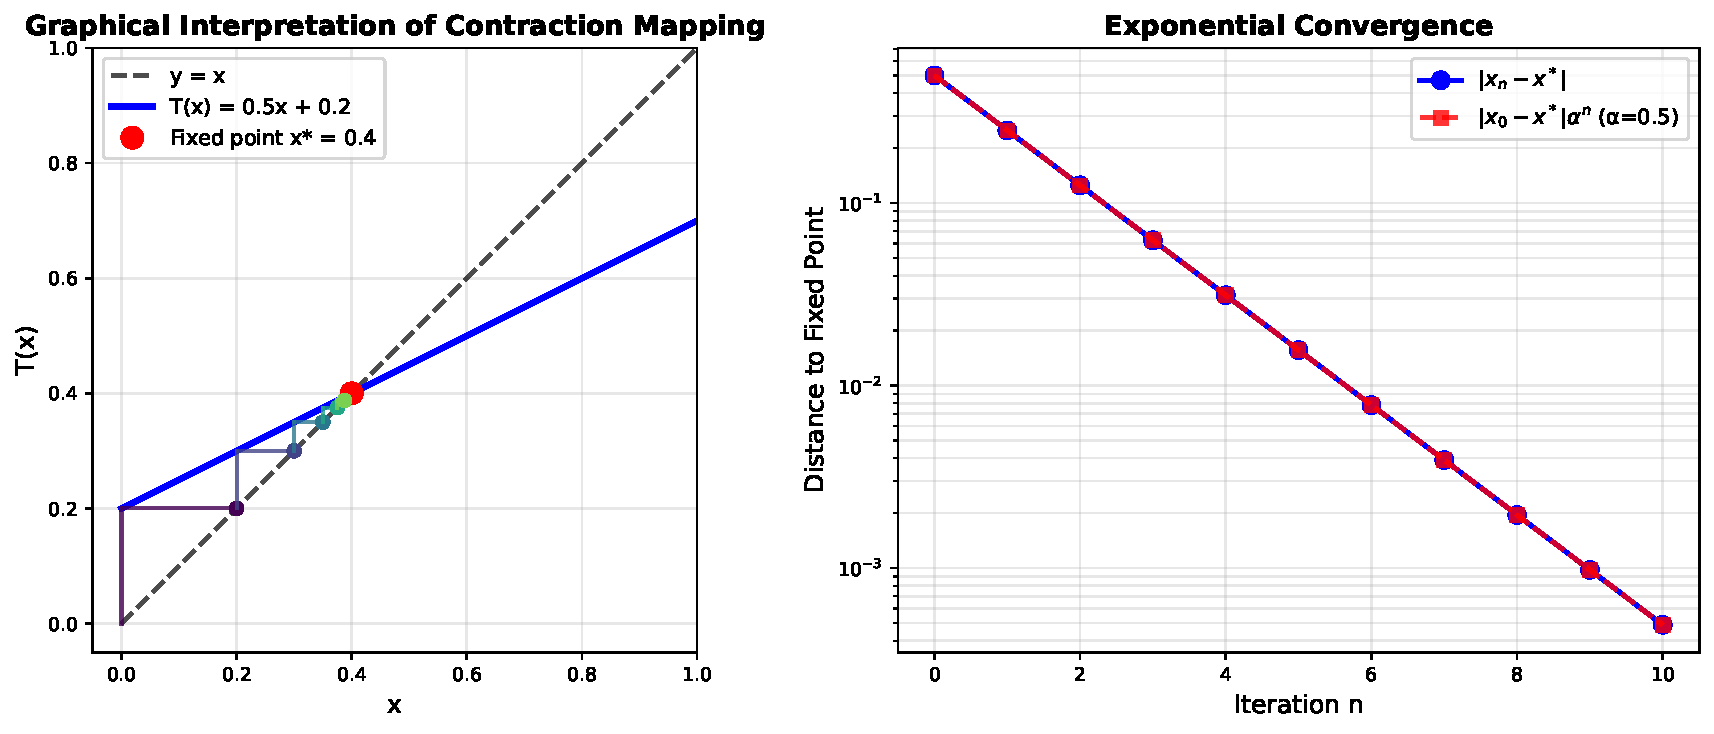
\includegraphics[width=\textwidth]{contraction_mapping.pdf}
    \end{center}

    \begin{itemize}
        \item \textbf{Left:} A contraction mapping can be visualized where the function curve is "steeper" than the identity line in some sense
        \item \textbf{Right:} Exponential convergence of errors with rate $\alpha$
    \end{itemize}
\end{frame}

\begin{frame}{Effect of Contraction Constant}
    \begin{center}
        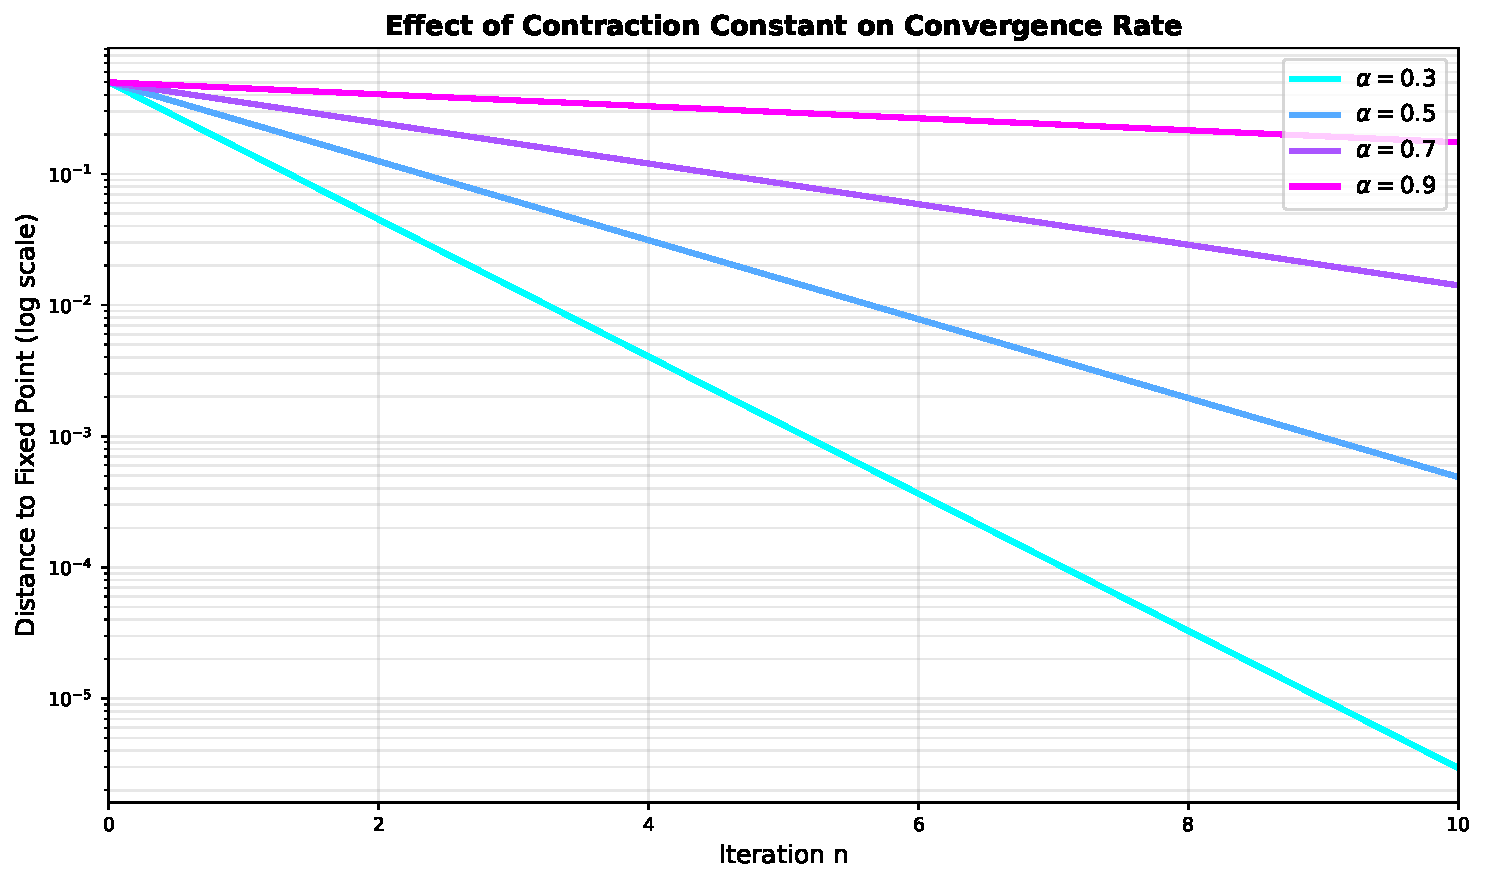
\includegraphics[width=\textwidth]{contraction_constant.pdf}
    \end{center}

    Key observations:
    \begin{itemize}
        \item Larger $\alpha$ (closer to 1) $\Rightarrow$ slower convergence
        \item Smaller $\alpha$ (closer to 0) $\Rightarrow$ faster convergence
        \item All exponential rates: $\alpha^n \to 0$ for $0 < \alpha < 1$
    \end{itemize}
\end{frame}

% Section 4: Banach Contraction Mapping Theorem
\section{Banach Contraction Mapping Theorem}

\begin{frame}[fragile]{Theorem Statement}
    \begin{theorem}[Banach Contraction Mapping Principle]
        Let $(X, d)$ be a \textbf{complete metric space} and let $T: X \to X$ be a \textbf{contraction mapping} with Lipschitz constant $\alpha \in (0,1)$. Then:

        \begin{enumerate}
            \item $T$ has a \textbf{unique fixed point} $x^* \in X$
            \item For any starting point $x_0 \in X$, the sequence $\{x_n\}$ defined by
                \[
                    x_{n+1} = T(x_n), \quad n = 0, 1, 2, \ldots
                \]
                converges to $x^*$
            \item The rate of convergence is exponential:
                \[
                    d(x_n, x^*) \leq \alpha^n d(x_0, x^*)
                \]
        \end{enumerate}
    \end{theorem}

    \vspace{0.3cm}
    \begin{center}
        \textcolor{blue}{\textbf{This is one of the most important and useful theorems in analysis!}}
    \end{center}
\end{frame}

\begin{frame}{Three Essential Conditions}
    \begin{center}
        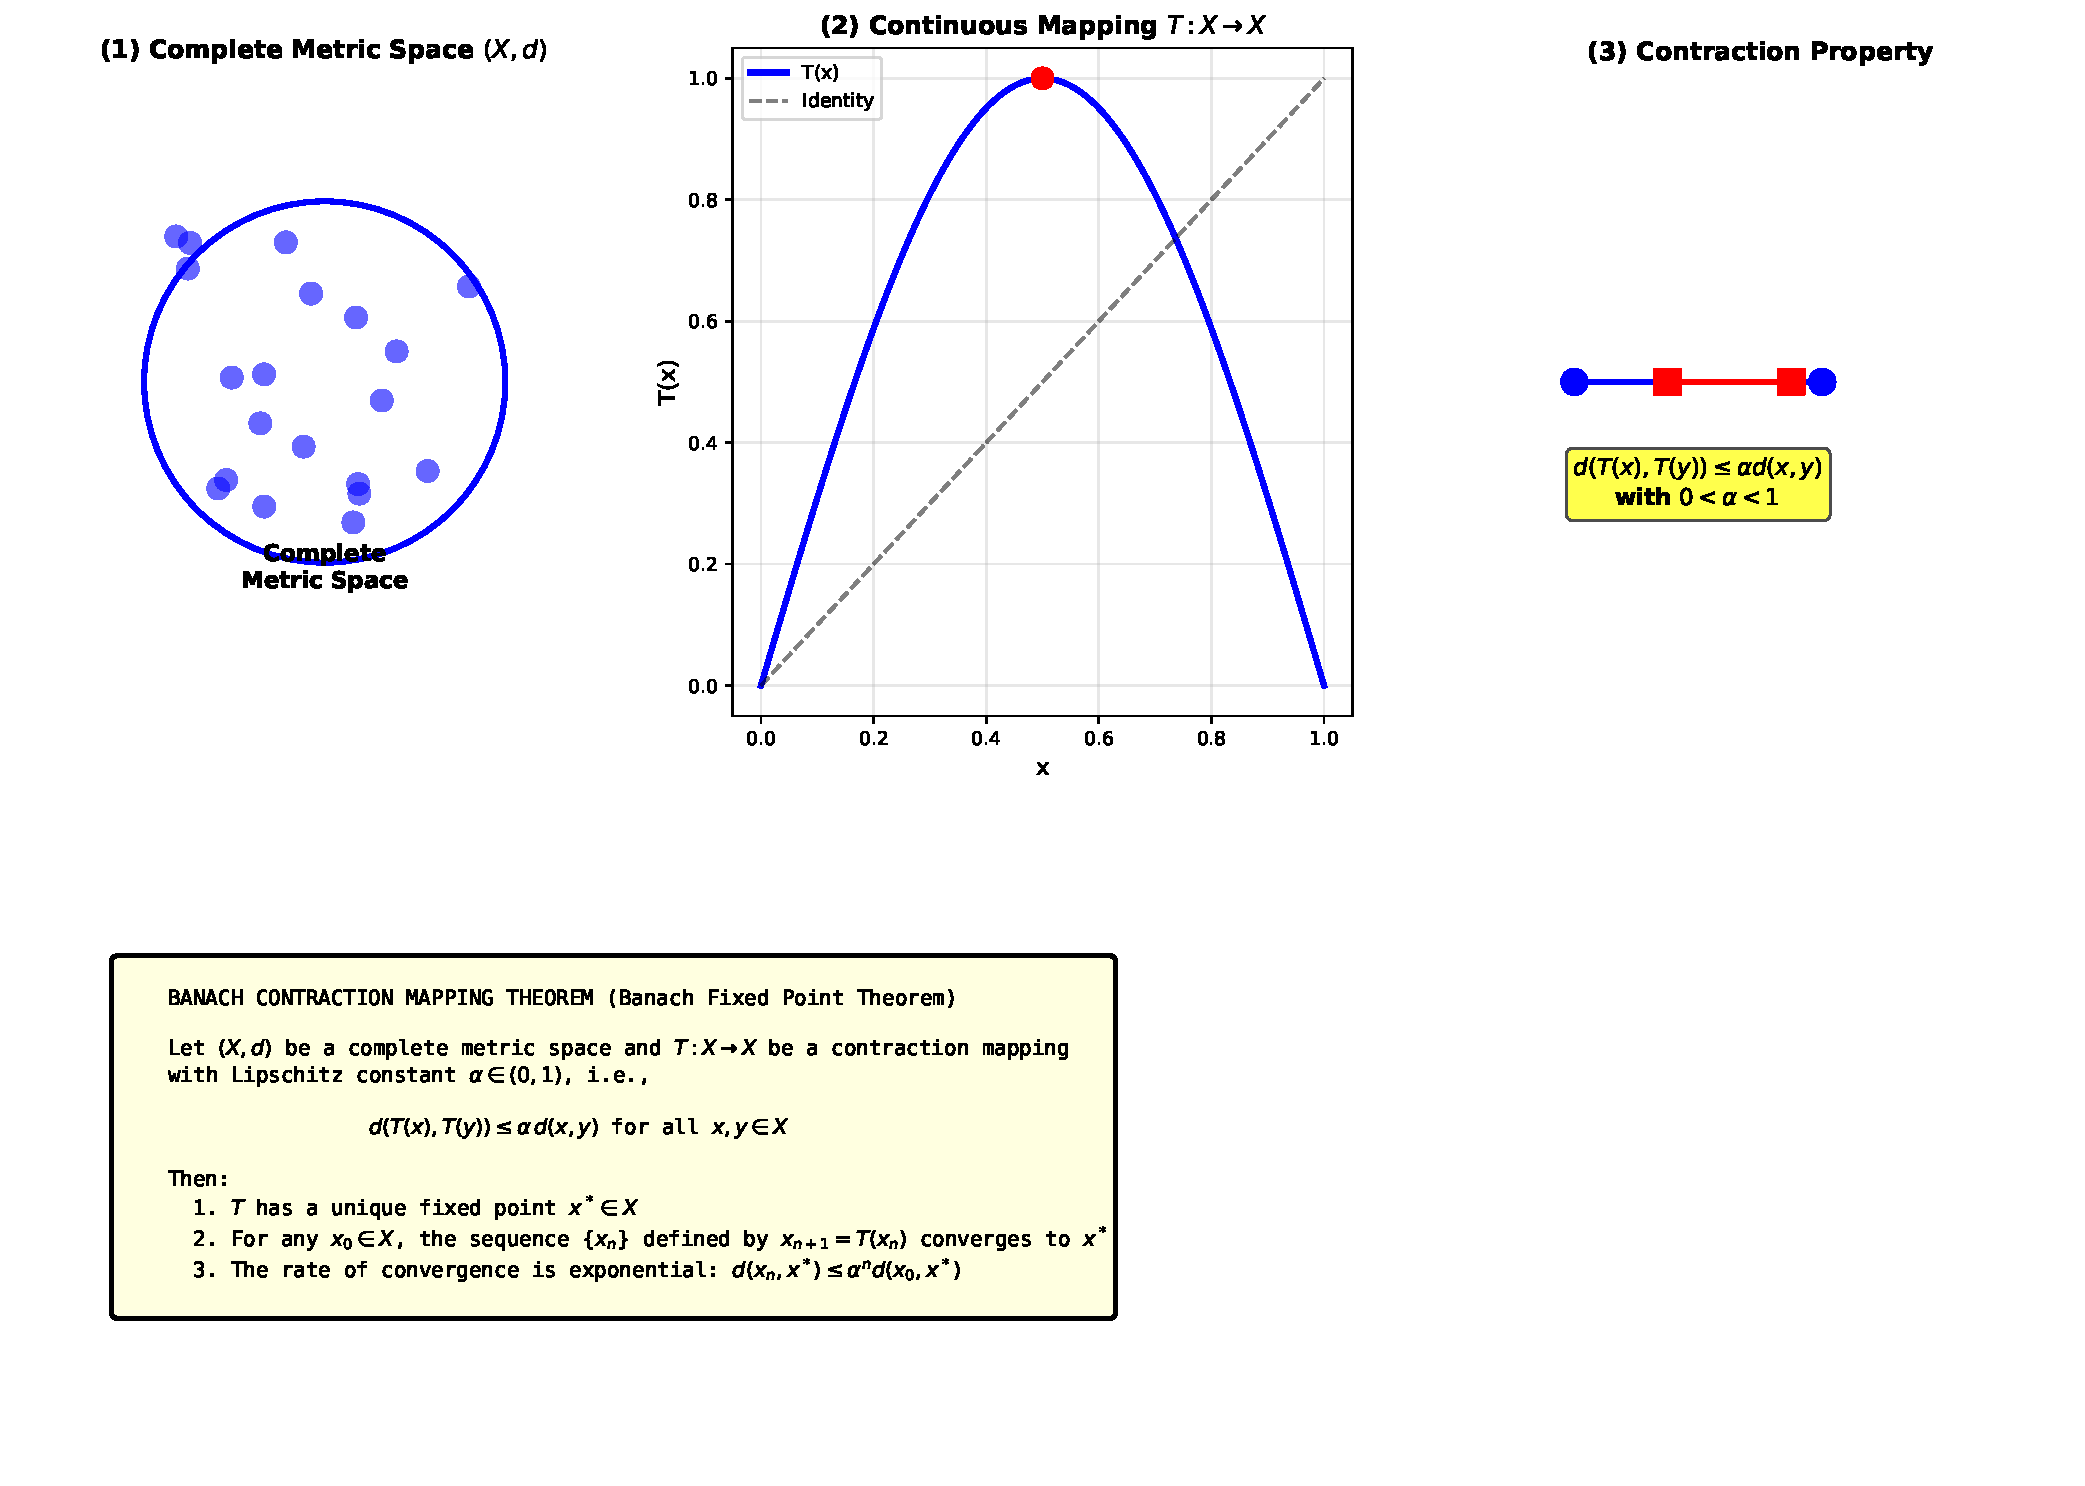
\includegraphics[width=\textwidth]{theorem_conditions.pdf}
    \end{center}

    The theorem requires:
    \begin{enumerate}
        \item Complete metric space
        \item Contraction mapping (with $\alpha < 1$)
        \item Domain: $T: X \to X$ (self-mapping)
    \end{enumerate}

    All three conditions are \textbf{necessary}!
\end{frame}

\begin{frame}{Proof Sketch}
    \begin{proof}[Sketch of Proof]
        \begin{enumerate}
            \item \textbf{Construction of sequence:} Starting from any $x_0 \in X$, define $x_{n+1} = T(x_n)$.

            \item \textbf{Cauchy property:} For $m > n$:
                \begin{align*}
                    d(x_m, x_n) &\leq d(x_m, x_{m-1}) + \cdots + d(x_{n+1}, x_n) \\
                                 &\leq \alpha^n(1 + \alpha + \cdots + \alpha^{m-n-1}) d(x_1, x_0) \\
                                 &\leq \frac{\alpha^n}{1-\alpha} d(x_1, x_0) \to 0
                \end{align*}

            \item \textbf{Convergence:} Since $(X,d)$ is complete and $\{x_n\}$ is Cauchy, $x_n \to x^*$ for some $x^* \in X$.

            \item \textbf{Fixed point:} By continuity of $T$:
                \[
                    T(x^*) = T(\lim_{n \to \infty} x_n) = \lim_{n \to \infty} T(x_n) = \lim_{n \to \infty} x_{n+1} = x^*
                \]

            \item \textbf{Uniqueness:} If $y^*$ were another fixed point, then
                \[
                    d(x^*, y^*) = d(T(x^*), T(y^*)) \leq \alpha d(x^*, y^*)
                \]
                This implies $(1-\alpha) d(x^*, y^*) \leq 0$, so $x^* = y^*$.
        \end{enumerate}
    \end{proof}
\end{frame}

% Section 5: Error Estimates and Convergence Analysis
\section{Error Estimation and Convergence}

\begin{frame}{Error Estimation Formulas}
    The Banach theorem provides explicit error bounds!

    \vspace{0.3cm}
    \begin{theorem}[Error Estimates]
        For the Picard iteration $x_{n+1} = T(x_n)$ with contraction $\alpha \in (0,1)$:

        \begin{enumerate}
            \item \textbf{A posteriori error bound:}
                \[
                    d(x_n, x^*) \leq \frac{\alpha}{1-\alpha} d(x_n, x_{n-1})
                \]

            \item \textbf{A priori error bound:}
                \[
                    d(x_n, x^*) \leq \alpha^n d(x_0, x^*)
                \]

            \item \textbf{Error reduction:}
                \[
                    d(x_n, x^*) \leq \frac{\alpha^n}{1-\alpha} d(x_1, x_0)
                \]
        \end{enumerate}
    \end{theorem}

    \vspace{0.3cm}
    These formulas allow us to:
    \begin{itemize}
        \item Estimate error without knowing the exact fixed point $x^*$
        \item Predict how many iterations needed for desired accuracy
        \item Design stopping criteria
    \end{itemize}
\end{frame}

\begin{frame}{Example: Convergence Analysis}
    \begin{center}
        
\includegraphics[width=\textwidth]{numerical_example.pdf}
    \end{center}

    Shows iteration table, convergence behavior, and error decay for $x = 0.8\cos(x)$.
\end{frame}

% Section 6: Picard Iteration Algorithm
\section{Picard Iteration Algorithm}

\begin{frame}{Picard Iteration Method}
    \begin{center}
        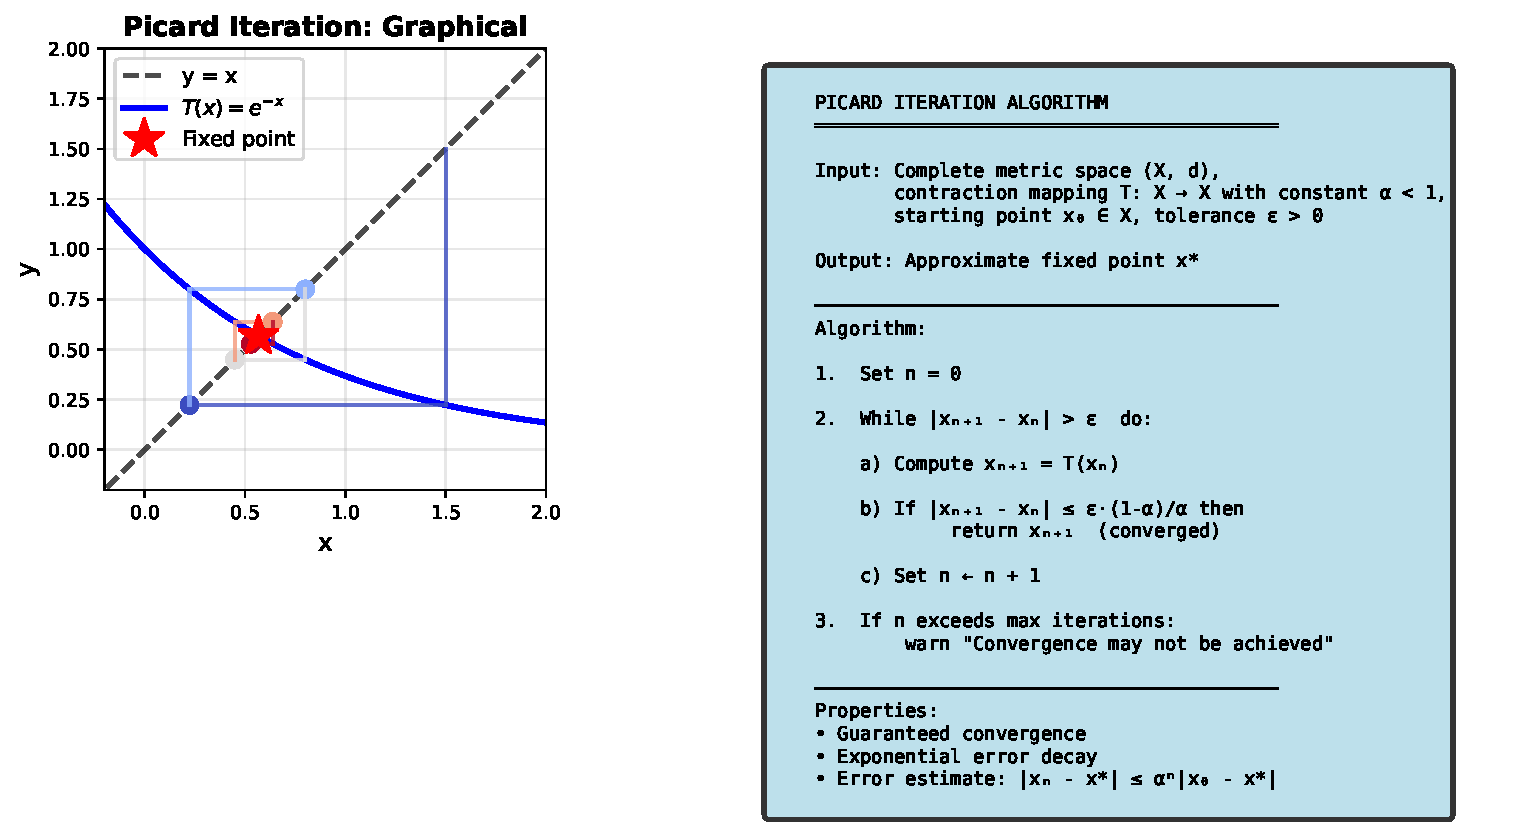
\includegraphics[width=0.9\textwidth]{picard_iteration.pdf}
    \end{center}
\end{frame}

\begin{frame}[fragile]{Implementation in Python}
    \begin{lstlisting}
def picard_iteration(T, x0, tol=1e-6, max_iter=100):
    # Picard iteration to find fixed point of T(x)
    x = x0
    errors = []

    for n in range(max_iter):
        x_new = T(x)
        error = abs(x_new - x)
        errors.append(error)

        if error < tol:
            return x_new, n+1, errors

        x = x_new

    print("Warning: Not converged after iterations")
    return x, max_iter, errors

# Example: Solve x = cos(x)
T = lambda x: np.cos(x)
x_star, n_iter, errors = picard_iteration(T, x0=0.5)

print("Fixed point:", x_star)
print("Iterations:", n_iter)
print("Final error:", errors[-1])
    \end{lstlisting}
\end{frame}

\begin{frame}{Convergence Behavior in Different Cases}
    \begin{center}
        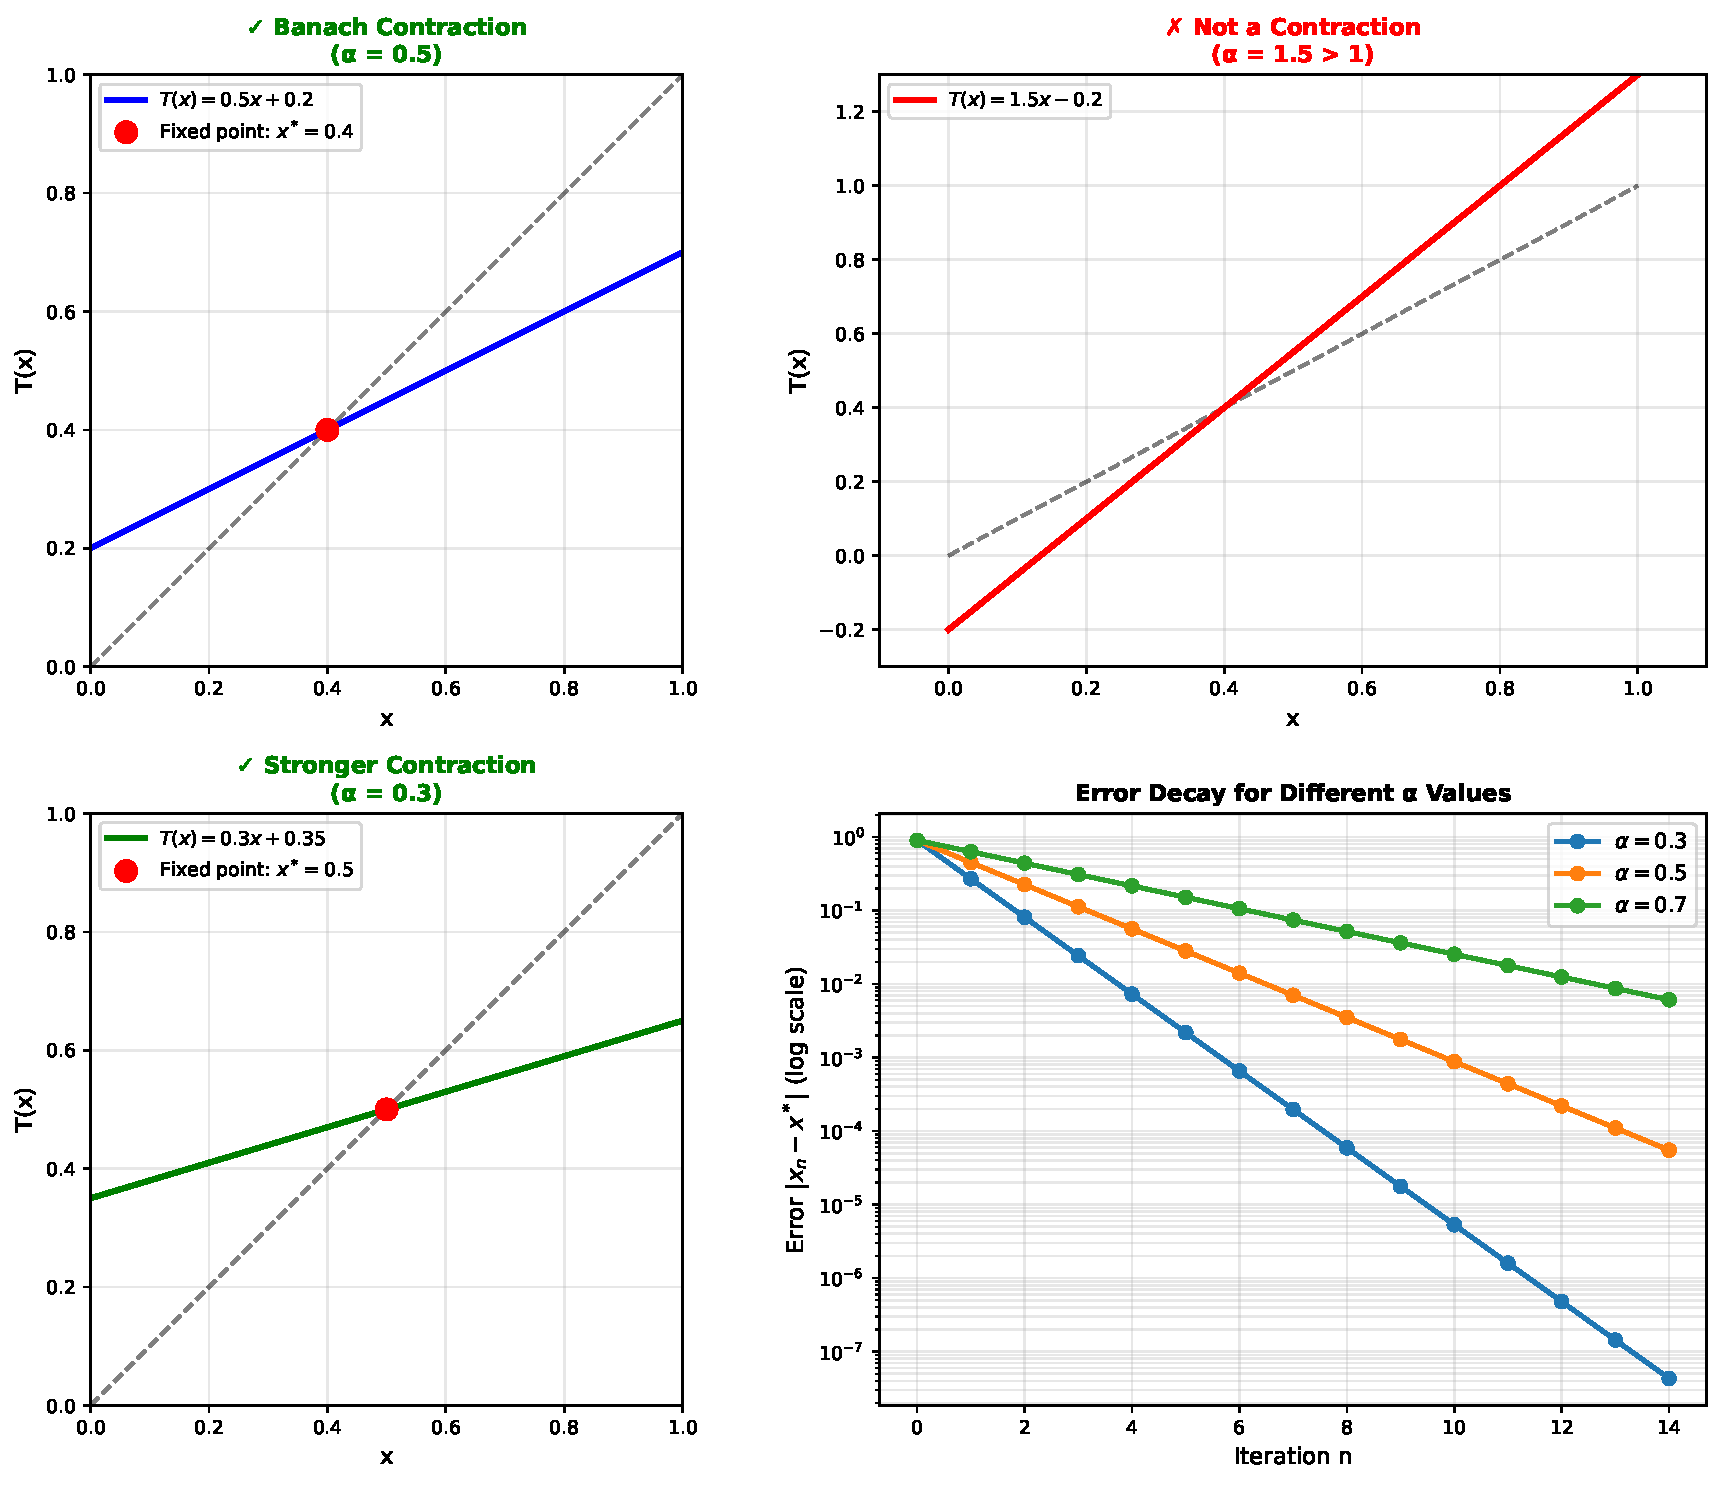
\includegraphics[width=\textwidth]{examples.pdf}
    \end{center}

    \begin{itemize}
        \item \textbf{Top left:} Banach contraction with $\alpha = 0.5$ (good!)
        \item \textbf{Top right:} Not a contraction, $\alpha > 1$ (diverges!)
        \item \textbf{Bottom left:} Stronger contraction with $\alpha = 0.3$ (faster!)
        \item \textbf{Bottom right:} Error decay for different $\alpha$ values
    \end{itemize}
\end{frame}

% Section 7: Applications
\section{Applications}

\begin{frame}{Application 1: Existence and Uniqueness for ODEs}
    \begin{theorem}[Picard-Lindelöf Theorem]
        Consider the initial value problem (IVP):
        \[
            y' = f(t,y), \quad y(t_0) = y_0
        \]

        If $f(t,y)$ is continuous in $t$ and \textbf{Lipschitz continuous in $y$} with constant $L$ (i.e., $|f(t,y_1) - f(t,y_2)| \leq L|y_1 - y_2|$), then on some interval $|t - t_0| \leq h$, there exists a \textbf{unique} solution $y(t)$.
    \end{theorem}

    \vspace{0.3cm}
    \begin{proof}[Idea]
        The IVP is equivalent to the integral equation:
        \[
            y(t) = y_0 + \int_{t_0}^t f(s, y(s)) \, ds
        \]

        Define $T: C([t_0, t_0+h]) \to C([t_0, t_0+h])$ by $(Ty)(t) = y_0 + \int_{t_0}^t f(s,y(s))\,ds$.

        The Lipschitz condition ensures $T$ is a contraction on an appropriate function space, so Banach's theorem guarantees existence and uniqueness!
    \end{proof}
\end{frame}

\begin{frame}{Application 2: Solving Nonlinear Equations}
    \begin{example}[Equation: $x = e^{-x}$]
        We want to solve $x = e^{-x}$, equivalently find the fixed point of $T(x) = e^{-x}$.

        \vspace{0.3cm}
        \begin{itemize}
            \item $T(x) = e^{-x}$ maps $\mathbb{R}$ to $(0, \infty)$
            \item On $[0, \infty)$: $|T'(x)| = e^{-x} \leq 1$
            \item On $[0, 1]$: $\sup_{x \in [0,1]} |T'(x)| = 1 \cdot e^{-0} = 1$
            \item But we need strict contraction for Banach theorem!

            \vspace{0.2cm}
            \item However, on $[0, 0.5]$: $|T'(x)| = e^{-x} \leq e^{-0} \approx 0.606 < 1$ (OK: contraction!)
        \end{itemize}

        \vspace{0.3cm}
        Using Picard iteration with $x_0 = 0.5$:
        \[
            x_1 = e^{-0.5} \approx 0.606, \quad x_2 \approx 0.544, \quad x_3 \approx 0.580, \cdots \to x^* \approx 0.567
        \]
    \end{example}
\end{frame}

\begin{frame}{Application 3: Integral Equations}
    \begin{example}[Hammerstein Equation]
        Consider the integral equation:
        \[
            x(t) = f(t) + \lambda \int_a^b K(t,s) \phi(s, x(s)) \, ds
        \]

        Define operator $T$ on $C([a,b])$ by:
        \[
            (Tx)(t) = f(t) + \lambda \int_a^b K(t,s) \phi(s, x(s)) \, ds
        \]

        If $\lambda$ is sufficiently small and $\phi$ is Lipschitz in the second argument, then $T$ is a contraction, and Banach's theorem guarantees unique solution.
    \end{example}

    \vspace{0.3cm}
    \begin{itemize}
        \item Volterra equations (convolution type)
        \item Fredholm equations (with small parameter)
        \item Urysohn equations
    \end{itemize}
\end{frame}

\begin{frame}{Application 4: Numerical Methods}
    \begin{itemize}
        \item \textbf{Newton-Raphson Method:} Can be viewed as fixed point iteration for $T(x) = x - \frac{f(x)}{f'(x)}$ (when it converges)

        \item \textbf{Successive Approximations:} For systems of equations

        \item \textbf{Iterative Solvers:} For linear systems $Ax = b$, rewrite as $x = x - \alpha(Ax - b)$ and choose $\alpha$ so that the resulting mapping is a contraction

        \item \textbf{Jacobi and Gauss-Seidel Methods:} Iterative solvers for linear systems
    \end{itemize}

    \vspace{0.3cm}
    The key advantage: \textbf{Explicit error bounds} and \textbf{guaranteed convergence} with quantified rate!
\end{frame}

% Section 8: Generalizations and Extensions
\section{Generalizations and Extensions}

\begin{frame}{Generalizations of Banach's Theorem}
    The classical Banach theorem has been extended in various directions:

    \vspace{0.3cm}
    \begin{itemize}
        \item \textbf{Quasi-contractions:} $d(Tx, Ty) \leq \alpha d(x,y) + L d(x, Tx) + L d(y, Ty)$

        \item \textbf{$\phi$-contractions:} $d(Tx, Ty) \leq \phi(d(x,y))$ where $\phi$ is increasing with $\phi(t) < t$ for $t > 0$

        \item \textbf{Weakly contractive:} $d(Tx, Ty) < d(x,y)$ for all $x \neq y$

        \item \textbf{Asymptotically regular:} $\|T^n(x) - T^{n+1}(x)\| \to 0$

        \item \textbf{Set-valued contractions:} Extensions to multifunctions

        \item \textbf{Coupled fixed points:} For systems of equations
    \end{itemize}

    \vspace{0.3cm}
    See Pathak's book Ch. 5 for detailed treatments of:
    \begin{itemize}
        \item Nonexpansive mappings
        \item Pseudocontractive mappings
        \item Asymptotically nonexpansive mappings
    \end{itemize}
\end{frame}

\begin{frame}{Comparison with Other Fixed Point Theorems}
    \begin{center}
        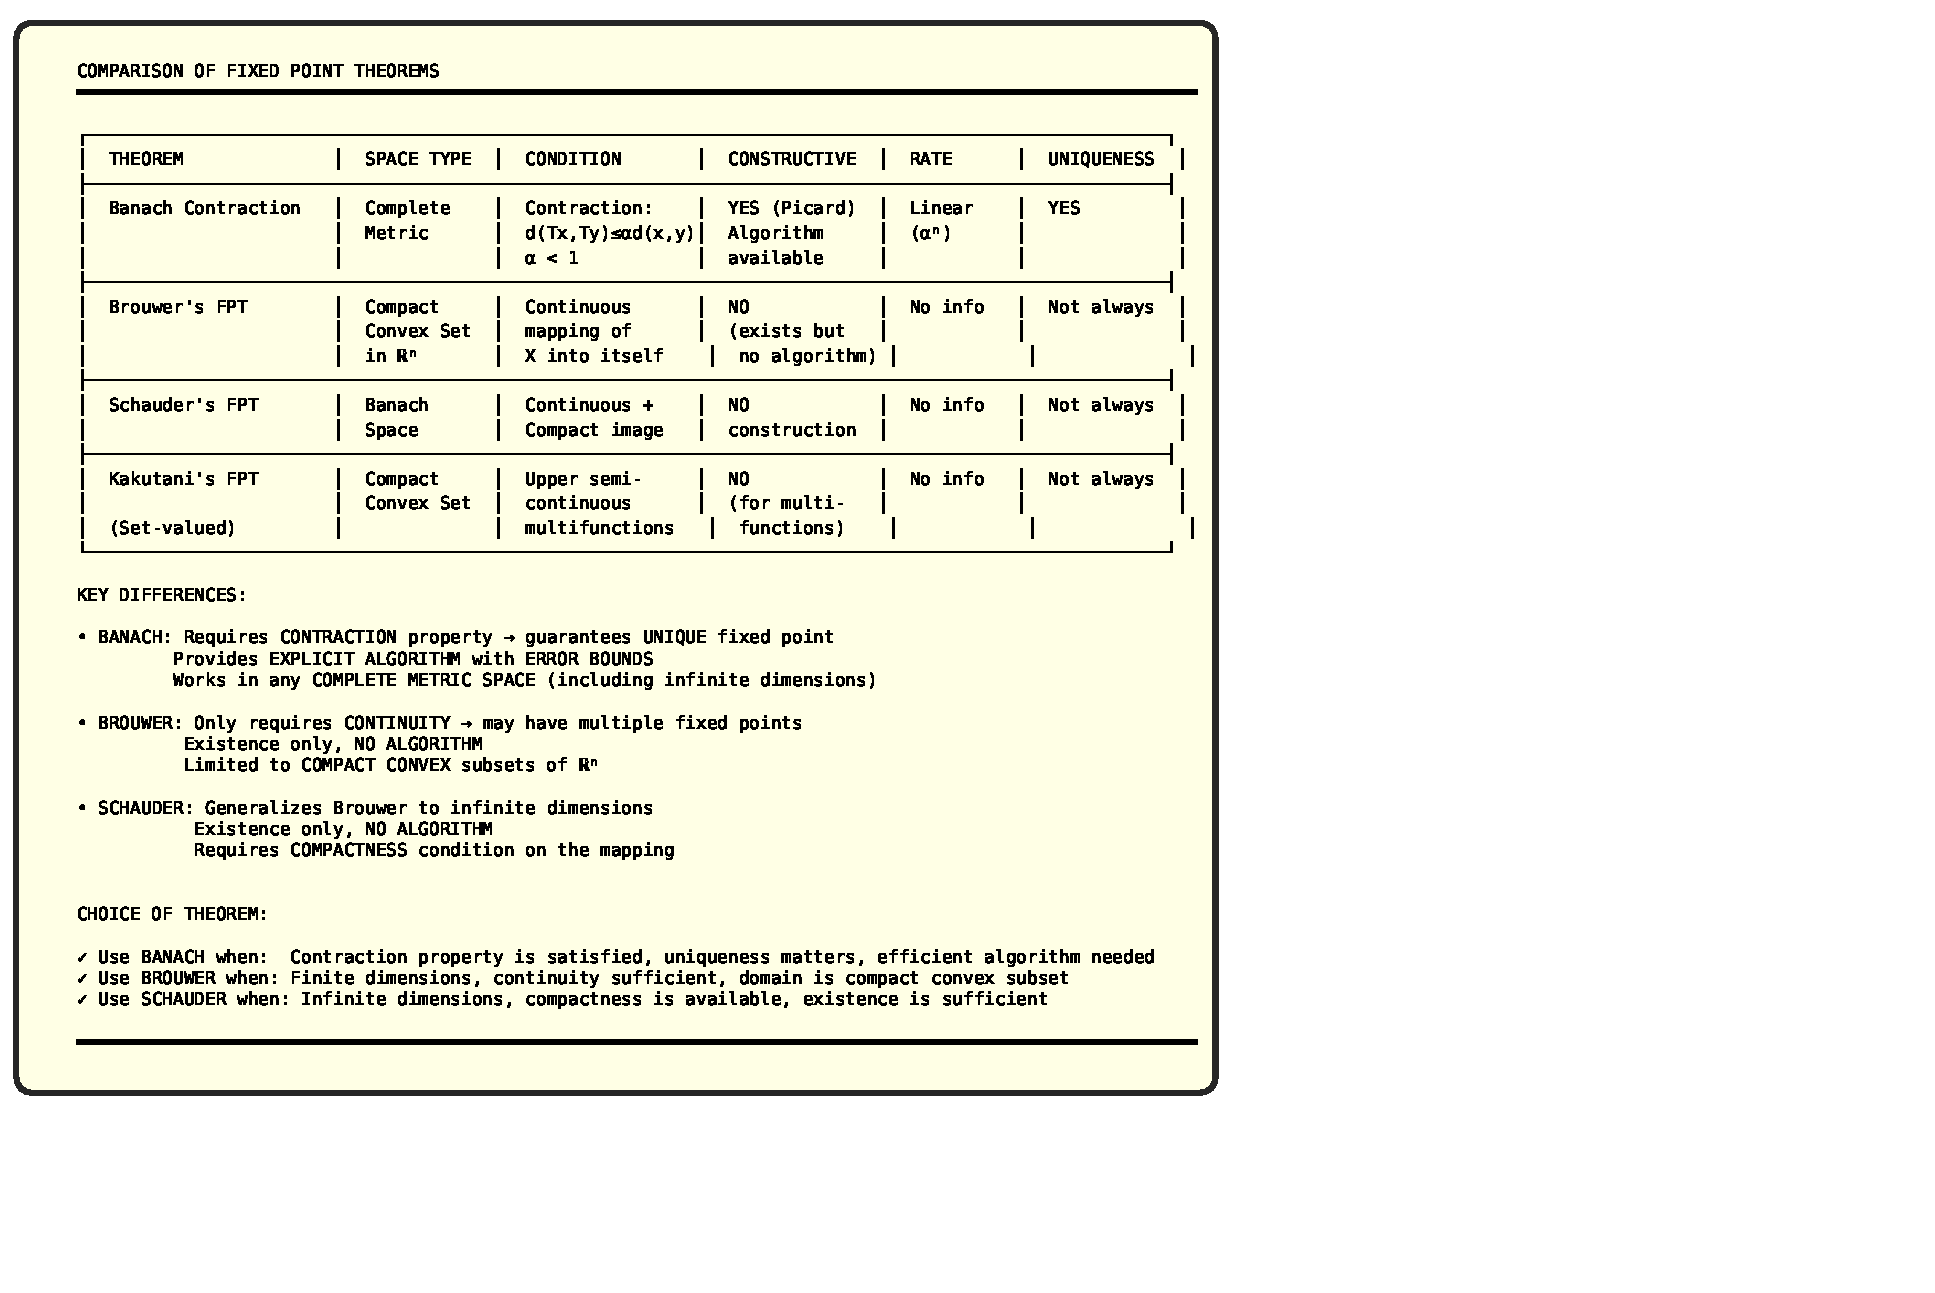
\includegraphics[width=\textwidth]{comparison_fixed_point_theorems.pdf}
    \end{center}
\end{frame}

\begin{frame}{When Does Banach Fail?}
    The Banach theorem requires the contraction condition $d(Tx, Ty) \leq \alpha d(x,y)$ with $\alpha < 1$.

    \vspace{0.3cm}
    \begin{example}[Continuous but not Contractive]
        Let $T: [0,1] \to [0,1]$ be defined by $T(x) = x/2$. Then:
        \begin{itemize}
            \item $T$ is continuous and has fixed point $x^* = 0$
            \item $T$ is a contraction with $\alpha = 1/2$
            \item So Banach applies! (OK)
        \end{itemize}
    \end{example}

    \vspace{0.3cm}
    \begin{example}[Continuous but NOT Contractive]
        Let $T: [0,1] \to [0,1]$ be the Brouwer example: $T(x) = \sqrt{x}$. Then:
        \begin{itemize}
            \item $T$ is continuous with fixed points $x^* = 0$ and $x^* = 1$
            \item $|T'(x)| = \frac{1}{2\sqrt{x}}$ unbounded as $x \to 0^+$
            \item So $T$ is NOT a uniform contraction
            \item But Brouwer's fixed point theorem still guarantees existence!
        \end{itemize}
    \end{example}
\end{frame}

% Section 9: Examples and Exercises
\section{Examples and Exercises}

\begin{frame}[fragile]{Example 1: Solving x = cos(x)}
    \begin{lstlisting}
import numpy as np

# Define the function and its derivative
T = lambda x: np.cos(x)
T_prime = lambda x: -np.sin(x)

# Check contraction on [0, pi/2]
alpha = np.max(np.abs(T_prime(np.linspace(0, np.pi/2, 100))))
print("Contraction constant alpha ~= ", alpha)

# Picard iteration
x = 0.5
for n in range(10):
    x_new = T(x)
    error = abs(x_new - x)
    print("x_%d = %f, error = %e" % (n, x, error))
    x = x_new

print("Fixed point:", x)
print("Verification: cos(x) =", np.cos(x))
    \end{lstlisting}
\end{frame}

\begin{frame}[fragile]{Example 2: System via Fixed Point}
    \begin{lstlisting}
import numpy as np

def T(z):
    x, y = z
    x_new = 0.5 * np.sin(x) + 0.5 * np.cos(y)
    y_new = 0.5 * np.cos(x) + 0.3 * x
    return np.array([x_new, y_new])

# Initial guess
z = np.array([0.5, 0.5])

# Iteration
for n in range(50):
    z_new = T(z)
    error = np.linalg.norm(z_new - z)
    if error < 1e-8:
        print("Converged at iteration", n)
        break
    z = z_new

print("Solution: x =", z[0], "y =", z[1])
print("Verification: T(z) =", T(z))
    \end{lstlisting}
\end{frame}

\begin{frame}{Exercise 1}
    \begin{exercise}
        Show that $T(x) = \frac{1}{2}\sin(x) + \frac{1}{4}$ is a contraction on $\mathbb{R}$.
        Find the contraction constant $\alpha$ and estimate the number of iterations needed to achieve
        accuracy $\varepsilon = 10^{-6}$ starting from $x_0 = 0$.
    \end{exercise}

    \vspace{0.3cm}
    \textbf{Solution hint:}
    \begin{enumerate}
        \item Find $\alpha = \sup_{x \in \mathbb{R}} |T'(x)| = \sup_{x \in \mathbb{R}} \frac{1}{2}|\cos(x)| = \frac{1}{2}$
        \item Use error estimate: $d(x_n, x^*) \leq \alpha^n d(x_0, x^*)$
        \item Need $\alpha^n < \varepsilon$, so $n > \frac{\log \varepsilon}{\log \alpha}$
        \item Compute: $n > \frac{\log 10^{-6}}{\log 0.5} \approx 19.93$, so $n \geq 20$ iterations
    \end{enumerate}
\end{frame}

\begin{frame}{Exercise 2}
    \begin{exercise}
        For the IVP $y' = y + t$, $y(0) = 1$, use Picard iteration to construct
        the first few approximations:
        \[
            y_n(t) = 1 + \int_0^t (y_{n-1}(s) + s) \, ds
        \]
        starting with $y_0(t) = 1$.
    \end{exercise}

    \vspace{0.3cm}
    \textbf{Solution:}
    \begin{align*}
        y_0(t) &= 1 \\
        y_1(t) &= 1 + \int_0^t (1 + s) \, ds = 1 + t + \frac{t^2}{2} \\
        y_2(t) &= 1 + \int_0^t (1 + s + \frac{s^2}{2} + s) \, ds = 1 + 2t + \frac{3t^2}{4} + \frac{t^3}{6} \\
        &\vdots \\
        y(t) &= e^t + t + 1 \quad \text{(exact solution)}
    \end{align*}
\end{frame}

\begin{frame}{Exercise 3}
    \begin{exercise}
        For $T(x) = 0.4x + 0.3$, find:
        \begin{enumerate}
            \item The fixed point $x^*$
            \item The contraction constant $\alpha$
            \item The number of iterations to reach $|x_n - x^*| < 10^{-10}$ starting from $x_0 = 0$
            \item The actual sequence $\{x_n\}$ for $n = 0, 1, \ldots, 10$
        \end{enumerate}
    \end{exercise}

    \vspace{0.3cm}
    \textbf{Solution:}
    \begin{enumerate}
        \item Fixed point: $x^* = 0.4x^* + 0.3 \Rightarrow x^* = \frac{0.3}{0.6} = 0.5$
        \item Contraction: $\alpha = |T'(x)| = 0.4$
        \item Iterations: $0.4^n \cdot 0.5 < 10^{-10} \Rightarrow n > \frac{\log(0.5 \times 10^{-10})}{\log 0.4} \approx 24.3$, so $n = 25$
        \item Sequence: $x_0 = 0$, $x_1 = 0.3$, $x_2 = 0.42$, $x_3 = 0.468$, $\ldots \to 0.5$
    \end{enumerate}
\end{frame}

% Section 10: Summary
\section{Summary}

\begin{frame}{Key Takeaways}
    \begin{enumerate}
        \item \textbf{Fixed Point Problem:} Find $x^*$ such that $T(x^*) = x^*$

        \item \textbf{Banach Theorem:} In a complete metric space, contractions have unique fixed points with exponential convergence

        \item \textbf{Constructive Method:} Picard iteration $x_{n+1} = T(x_n)$ provides explicit algorithm

        \item \textbf{Error Bounds:} Explicit formulas allow us to estimate errors without knowing $x^*$

        \item \textbf{Applications:} Existence/uniqueness for ODEs, integral equations, numerical methods, etc.

        \item \textbf{Necessity of Conditions:} All three conditions (complete space, contraction, self-mapping) are essential

        \item \textbf{Generalizations:} Extended to weaker conditions, set-valued mappings, infinite dimensions
    \end{enumerate}

    \vspace{0.3cm}
    \begin{center}
        \textcolor{red}{\textbf{The Banach Contraction Mapping Theorem is a cornerstone of analysis and numerical mathematics!}}
    \end{center}
\end{frame}

\begin{frame}[allowframebreaks]{References}
    \begin{thebibliography}{99}
        \bibitem{pathak2018} Pathak, H. K. (2018). \textit{An Introduction to Nonlinear Analysis and Fixed Point Theory}. Springer.

        \bibitem{banach1922} Banach, S. (1922). Sur les opérations dans les ensembles abstraits et leur application aux équations intégrales. \textit{Fundamenta Mathematicae}, 3(1), 133-181.

        \bibitem{rus2005} Rus, I. A. (2005). Picard operators and applications. \textit{Scientiae Mathematicae Japonicae}, 58(1), 191-219.

        \bibitem{granas1982} Granas, A., \& Dugundji, J. (1982). \textit{Fixed Point Theory}. Springer-Verlag.

        \bibitem{deimling1985} Deimling, K. (1985). \textit{Nonlinear Functional Analysis}. Springer-Verlag.

        \bibitem{kirk2001} Kirk, W. A., \& Sims, B. (Eds.). (2001). \textit{Handbook of Metric Fixed Point Theory}. Kluwer Academic Publishers.
    \end{thebibliography}
\end{frame}

\begin{frame}{Additional Resources}
    \begin{itemize}
        \item Pathak, H. K. (2018). Chapter 5: Fixed Point Theorems - detailed treatment of contractions and generalizations

        \item Online courses: MIT 18.100 (Real Analysis), Stanford CME 100 (Scientific Computing)

        \item Interactive visualizations: Fixed point iteration applets, Desmos graphing

        \item Numerical algorithms: Implementation in Python (scipy.optimize), MATLAB

        \item Applications: Numerical methods textbooks (Burden and Faires, Atkinson)
    \end{itemize}
\end{frame}

\end{document}
